\section{Generalidades}
Los textos son, por mucho, las estructuras de datos más utilizadas en
la computación.  Toda operación en una computadora implica algún
procesamiento de texto.  Por ejemplo:

\begin{itemize}
\item Compilar un programa: significa procesar un texto de entrada,
  que es el programa fuente, hecho en algún lenguaje de programación
  legible para los humanos, para producir un texto de salida: un
  programa binario, que legible para la computadora, que aunque el
  humano no lo puede leer directamente, sigue siendo un texto
\item Procesador de palabras: lee del teclado, letras y comandos que
  generarán un texto.  En estos programas usualmente hay muchas
  operaciones adicionales sobre los textos como la verificación de
  ortografía, formateo de la impresión, etc.
\end{itemize}

En general, los textos se utilizan en todos las aplicaciones que
exista comunicación entre dispositivos, entre computadoras, entre
computadoras y personas.

Claro que cuando hablamos de textos como estructura de datos, ya no
estamos hablando de contenedores mapas, como árboles y tablas, ya que
no hay elementos de un mismo tipo que se puedan acceder por una llave.

Los textos son estructuras de datos, ya que se trata de conjuntos de
datos semánticamente relacionados, con la cual se pueden realizar
distintas operaciones y transformaciones.  También existen diferentes
formas de representación que influirán en el desempeño de una
aplicación.

\begin{quote}
  \textbf{Texto}

  Secuencia de caracteres de longitud finita, que se usa para
  representar información semánticamente relacionada.
\end{quote}

Nótese que esta definición acepta desde los textos legibles por
humanos, programas ejecutables y paquetes de transmisión en la red.

\subsection{Representaciones}
\label{sec:representaciones}

Normalmente estamos acostumbrados a una sólo representación de textos,
que es la representación contigua con \textbf{codificación de longitud
  fija}, como la codificación ASCII o la UNICODE.  Sin embargo veremos
que existen otras codificaciones, no necesariamente contiguas y donde
el número de bits utilizado para representar cada caracter puede
variar de caracter a caracter.

\subsection{Operaciones}
\label{sec:operaciones}

Cuando se habla de operaciones sobre textos o strings, inmediatamente
pensamos en catenación, eliminación de caracteres o inserción de
caracteres.  Sin embargo éstas no son las únicas operaciones que
podemos hacer en un texto, y, sin darnos cuenta, las realizamos en
muchas aplicaciones de la vida diaria.

Las operaciones que vamos a estudiar son:

\begin{description}
\item[Encriptación: ] Transformación de un texto legible en uno
  ilegíble (criptograma) que sólo puede ser interpretado por quien
  tenga una palabra oculta (contraseña)
\item[Búsqueda de patrones: ] Consiste en buscar dentro de texto si
  existe o no una palabra determinada (patrón) y, si existe,
  determinar la posición o posiciones donde se encuentra.
\item[Macroexpansión: ] Consiste en expandir un abreviatura de un
  texto, a otro texto basado en parámetros. Por ejemplo: lo que
  realiza el precompilador de C/C++ con las directivas \#define.
\item[Compresión: ] Es la transformación que consiste en representar
  un texto en menos espacio que en su representación normal.
\end{description}

\section{Búsqueda de patrones}
\label{sec:busqueda-de-patrones}

La búsqueda de patrones es una de las operaciones más comunes a
realizar en los textos en cualquier aplicación.

La operación básica es que se tiene un texto de $n$ caracteres $S[n]$
y un texto de $m$ caracteres $p[m]$, donde $m \leq n$, y se desea
determinar si $p[m]$ forma parte de $s[n]$, y si es así determinar la
posición dentro de $s[n]$ donde se encuentra.

Existen diferentes métodos para realizar esta operación:
\begin{itemize}
\item Búsqueda simple o de fuerza bruta
\item Booyer Moore
\item Knutt Morris Pratt
\end{itemize}
Las cuales detallaremos a continuación.

\subsection{Búsqueda simple o de fuerza bruta}
\label{sec:busqueda-simple-o}

Es el método en el cual se compara directamente caracter a caracter
cada una de las posiciones de $p[m]$ en $s[n]$.  Se puede realizar con
el siguiente algoritmo:

\begin{verbatim}
int buscar (char *p, char *s, int m, int n) {
    while (i <= n-m && !encontrado)
    {          
        j = 1 ;
        while (j <= m && i+j-1<=n && s[i+j-1] == p[j])
            j ++ ;
        i ++ ;
        encontrado = (j > m) ;
    }

    return encontrado?i:-1 ;
}
\end{verbatim}

Si vemos el proceso como una sucesión de superposiciones de s[n] y
p[m], la ejecución del algoritmo, sobre s[10]=''HOLALALASA'' y
p[5]=''LALAS'' puede verse así:

\begin{verbatim}
\end{verbatim}

\begin{alltt}
  H O L A L A L A S A

  {\bf L} A L A S

  {\bf L} A L A S

  {\bf L A L A S}

  {\bf L} A L A S

  {\bf L} A L A S <---- encontrado
\end{alltt}

La letra negrilla indica el caracter de p[m] que se compara con la
posición superpuesta de s[n] y el subrayado indica la comparación que
falla.

El rendimiento de éste algoritmo es de \textbf{n*m} ya que en el peor
de los casos se compararán todas las posiciones de p contra s, por
ejemplo: si s[9]=''LALALALAS'' y p[3]=''LAS''

Ejercicio: demostrar que el O(buscar(n,m)) = n*m

\subsection{Boyer Moore y Knutt Morris Pratt}
\label{sec:boyer-moore-y}
\href{http://users.dcc.uchile.cl/~bebustos/apuntes/cc30a/BusqTexto/}{Búsqueda
  en texto.}

\section{Encripción}
\label{sec:encripcion}

La encripción es una operación sobre textos que consiste en una
transformación de un texto legible, para transformarlo en un texto
ilegible, que pueda ser transmitido por un medio público sin que pueda
ser descifrado, sino hasta que llegue al destinatario, quien podrá
aplicar la transformación inversa y obtener el texto original.

Este proceso se ilustra en la siguiente gráfica:

\begin{center}
  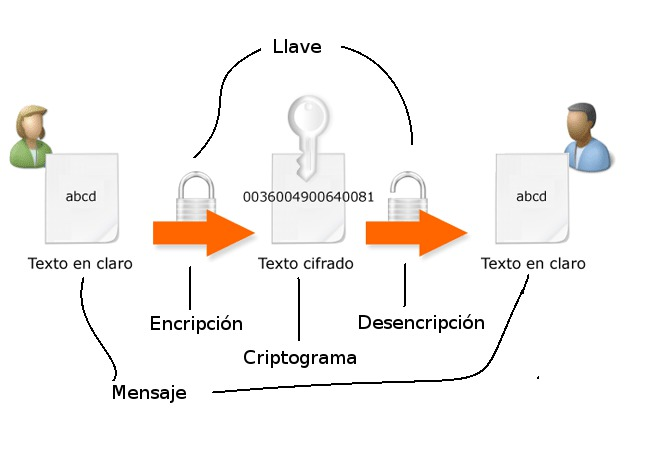
\includegraphics[scale=.7]{1textos.jpg}
\end{center}

Como podemos apreciar, hay varios elementos involucrados:
\begin{description}
\item[Mensaje: ] Es el texto legible para cualquier persona
\item[Llave: ] Es una palabra o contraseña secreta, que sólo sabe el
  remitente y el destinatario del mensaje
\item[Encripción: ] Es la operación de transformar el texto en claro,
  utilizando la llave, en un texto ilegible
\item[Criptograma: ] es el texto ilegible, resultado de la operación
  de encripción
\item[Desencripción: ] Es la operación de transformar el criptograma
  en el texto original, utilizando la llave predeterminada.
\end{description}

Mas formalmente podemos decir que la encripción es:

\begin{quote}
  Si se tiene un texto T y una clave K, se puede aplicar una función
  de encripción E(T,K) = C, donde C se llama criptograma, al cual se
  le puede aplicar una función de desencripción D(C,K) = T para
  obtener el texto original
\end{quote}

El uso de la encripción viene desde los inicios de la historia, desde
que las personas han deseado la privacidad, pero la aplicación
principal ha sido la guerra.

Los espartanos, son de los primeros que se sabe hacían uso de la
encripción en el Siglo V AC, empleando cintas de lino y un bastón
llamado escitalo. La cinta se enrollaba en el bastón y se escribía el
texto transversalmente en el bastón, tal como se muestra en la
siguiente gráfica:

\begin{center}
  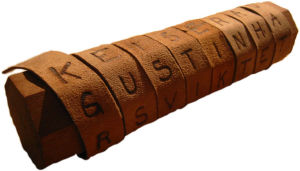
\includegraphics{2textos.jpeg}
\end{center}

El mensajero se le entregaba la cinta, la cual al extenderla era
ilegible.  Para descifrarla, el destinatario debería tener un bastón
del mismo diametro, enrollar la cinta, y leer la sección transversal
que tuviera sentido.  Este tipo de encripción es lo que actualmente se
llama \textbf{transposición}, porque se cambia de sitio los símbolos
del mensaje original

En Roman, Julio César desarrolló un mecanismo de codificación que
lleva su nombre.  Consiste en la \textbf{sustitución} de cada letra
por la que aparece tres posiciones a su derecha en el alfabeto, así la
A se convierte en D, la B en E y así sucesivamente.  Ejemplo:

\begin{quote}
  JUAN -> KVBO (corrimiento de 1 caracter)
\end{quote}

Otro método más moderno es la \textbf{confusión} u
\textbf{ofuscación}, que consiste en ocultar mensajes dentro de otro
mensaje claro.  Ejemplo de ésto es lo que comunmente se llama ''leer
entre líneas''.  Por ejemplo:

\begin{alltt}
  Éste es un mensaje

  en el cual no hay nada

  oculto entre

  este mensaje y

  otro mensaje que

  aunque es peligroso

  parece inofensivo

  y puede representar

  ante los que no sepan leer

  la sabiduría que está

  entre líneas.
\end{alltt}

Leer este mensaje de forma normal no releva nada claro, pero si leemos
las líneas impares podremos leer el mensaje ''\textit{Éste es un
  mensaje oculto entre otro mensaje que parece inofensivo ante los que
  no sepan leer entre líneas}''.

La \textbf{estenografía}, aunque algunos autores no la consideran
encripción en sí, es un método que aprovecha los vacíos que se dan
entre los diferentes formatos de gráficos y multimedios para ocultar
información.  Por ejemplo en el formato jpg hay espacios que no se
utilizan como parte de la gráfica que representa, por lo tanto, dichos
espacios pueden ser utilizado para poner información.  Lo mismo sucede
con el formato \textbf{mp3}, y otros formatos de música y gráficos.

Claro que en la computación moderna, éstos métodos distan mucho de ser
efectivos, ya que serían fácilmente descifrados.  Actualmente se han
desarrollado una gran cantidad de algoritmos y métodos de encripción,
los cuales clasificaremos en dos grupos:

\begin{enumerate}
\item encripción simétrica o privada
\item Encripción asimétrica o pública
\end{enumerate}

\subsection{Encripción simétrica o privada}
\label{sec:encr-simetr-o}

Es el primer tipo de encripción moderno trabajado a nivel
computacional, incluyen máquinas como la máquina codificadora
\textbf{Enigma}, durante la Segunda Guerra Mundial, en el cual la
misma llave utilizada para encriptar, es la que se necesita para
realizar la desencripción. Un ejemplo simple es la mezcla con
secuencias fijas aleatorias, en la cual se aprovecha la siguiente
propiedad de la operación xor

sea x \& y dos enteros independientes, entonces se cumple que
\begin{itemize}
\item (x xor y) xor x = y
\item (x xor y) xor y = x
\end{itemize}

Si T es el texto a encriptar, T se ve como una secuencia de enteros
$T_1T_2T_3...T_n$.  La llave secreta K, también se ve como una
secuencia de enteros $K_1K_2K_3...K_m$, donde m $\leq$ n.  El
criptograma C, visto como $C_1C_2C_3...C_n$ se forma por sucesivas
operaciones xor, de superposiciones de la llave K sobre el texto T,
así:

\[
\begin{array}{|cccccccccc|}
  \hline
  T   & T_1 & T_2 & ... & T_m & T_{m+1} & T_{m+2} & ... & T_{n-1} & T_n \\ 
  &    &    &     &  xor &      &      &     &      &      \\
  K   & K_1 & K_2 & ... & K_m & K_1   & K_2   & ... & K_i   & K_{i+1} \\
  &    &    &     &  =   &      &      &     &      &      \\
  C   & C_1 & C_2 & ... & C_fm & C_{m+1} & C_{m+2} & ... & C_{n-1} & C_n \\
  \hline
\end{array}
\]

y la operación de desencripción sería así:

\[
\begin{array}{|cccccccccc|}
\hline
  C   & C_1 & C_2 & ... & C_m & C_{m+1} & C_{m+2} & ... & C_{n-1} & C_n\\
       &    &    &     &    & xor     &      &     &      &      \\
  K   & K_1 & K_2 & ... & K_m & K_1   & K_2   & ... & K_i   & K_{i+1}\\
      &    &    &     &    &  =    &      &     &      &      \\
  T   & T_1 & T_2 & ... & T_m & T_{m+1} & T_{m+2} & ... & T_{n-1} & T_n\\
\hline
\end{array}
\]

Una encripción simple y eficiente, pero en una combinatoria de $16^m$
puede encontrarse la llave K (suponiendo que 16 bits es el tamaño de
un entero).

Entre los algoritmos de encripción simétrica actuales se encuentran:

\begin{itemize}
\item DES (Data Encryption Standard): llave de 56 bits de longitud,
  tiempo menor a 3 meses para desencriptar el mensaje
\item Triple – DES
\item Advanced Encryption Standard  (AES)
\item Blowfish
\end{itemize}
    
A pesar de la importancia que han tenido (y seguirán teniendo) la
encripción simétrica, en nuestro mundo actual de comunicación masiva y
globalizada, tener comunicación privada, a través de estos métodos,
presentan dos problemas importantes:

\begin{description}
\item[La paradoja del canal seguro: ] si deseamos encriptar un
  mensaje, es porque seguramente debemos enviarlo a través de un medio
  o canal que se considera inseguro, como el correo electrónico.  El
  problema se deriva que el destinatario está geográficamente distante
  y no es posible enviarla la contraseña por un medio seguro, y si
  hubiera un medio seguro, no sería necesario encriptar el mensaje
\item[La multiplicidad de intercambios: ] Si 2 personas necesitan
  comunicación privada, deben realizar un intercambio de llaves.  Si
  son 3 personas, deben realizar un total de 6 intercambios (2 por
  cada participante), sin son 4, 12 intercambios y así sucesivamente,
  que resulta en que si \textbf{n} personas desean comunicarse
  privadamente, deben haber \textbf{n*(n-1)} intercambios, lo que
  representa un órden cuadrático.
\end{description}

Estos problemas hicieron que la encripción simétrica fuera
insuficiente para lograr una comunicación privada eficiente en el
Internet, y es allí donde cobra importancia la encripción asimétrica.

\subsection{Encripción asimétrica o pública}
\label{sec:encr-asim-o}

El RSA es el criptosistema de llave pública más popular basado en el
modelo de Diffie-Hellman, el cual ofrece encripción y firmas digitales
(autentificación). Ron Rivest, Adl Shamir y Leonard Adleman
desarrollaron el RSA en 1977, de ahí su nombre formado por la primera
letra del apellido de sus inventores.

La base de este sistema es la compleja matemática detras de la
factorización de números primos grandes (ver links publicados), que
van desde 128 bits hasta 1024, lo cual está fuera del alcance del
curso.  Sin embargo, lo importante de este método es que tiene las
siguientes propiedades:

\begin{enumerate}
\item Cada usuario tiene dos llaves, una privada y otra pública.  La
  llave privada es conocida sólo por el propietario y normalmente es
  almacenada en un archivo protegido por una llave simétrica, conocida
  sólo por el dueño.  La llave pública, por el contrario debe ser
  conocida por todos los posibles destinatarios, y generalmente se
  publica por cualquier canal inseguro (correo electrónico, redes
  sociales, directorio públicos, etc)
\item Sea
  \begin{enumerate}
  \item T el texto o mensaje en claro
  \item $X_{prv}$ la llave privada de la persona X
  \item $X_{pbl}$ la llave pública de X
  \item C=E(T,K) la función de encripción del texto T con la llave K,
    que da como resultado el criptograma C
  \item T=D(C, K) la función de desencripción del criptograma C, con
    la llave K, que da como resultado el texto T
  \item Entonces, para RSA se cumple que:
    \begin{enumerate}
    \item si C=E(T, $X_{prv}$) entonces T=D(C, $X_{pbl}$), es decir lo que se
      encripta con la llave privada, sólo puede desencriptarse con la
      llave pública
    \item si C=E(T,$X_{pbl}$ entonces T=D(C, $X_{prv}$), es decir los que se
      encripta con la llave pública, sólo puede desencriptase con la
      llave privada
    \end{enumerate}
  \end{enumerate}
\end{enumerate}

Estas propiedades eliminan los problemas de la paradoja del canal
seguro, por el uso de la llave pública, y la multiplicidad de
intercambios, ya que para que n personas se comunican, sólo se
necesitan n intercambios de llaves públicas.

Además ya se puede realizar una comunicación privada así:
\begin{itemize}
\item Si X envía un mensaje a Y, encriptado con $X_{prv}$, Y lo
  desencriptará con $X_{pbl}$, con lo cual Y estará seguro que X es el
  remitente, ya que el mensaje fue encriptado con $X_{prv}$
\item Si X envía un mensaje a Y, encriptado con Ypbl, Y lo
  desencriptará con Yprv, con lo cual X estará seguro que sólo Y podrá
  leerlo, ya que sólo Y conoce Yprv
\item Al combinar ambos mecanismos, X puede crear un criptograma, en
  el cual se X se asegure que sólo Y puede verlo y Y estará seguro que
  X es el remitente, así:
  \begin{itemize}
  \item X encriptará así:
    \begin{itemize}
    \item $C_1$ = E (T, $X_{prv}$)
    \item $C_2$ = E ($C_1$, Ypbl)
    \end{itemize}
  \item Se envía $C_2$ a Y
  \item Y desencriptará así:
    \begin{itemize}
    \item $C_1$= D ($C_2$, Yprv)
    \item T = D ($C_1$, $X_{pbl}$)
    \end{itemize}
  \end{itemize}
\end{itemize}

Estas propiedades han hecho de RSA la base de todos los protocolos de
seguridad que conocemos, como PGP, HTTP, SSL, etc.  Sin embargo,
debido a su complejidad matemática, que involucra operaciones de
exponentes y módulos con número grandes (de hasta 1024 bits o sea
$2^{1024}$), su rendimiento es mucho menor que el de un algoritmo
simétrico.  Por lo tanto, los protocolos mencionados, hacen una
combinación de métodos simétricos y asimétricos, en los que éstos
últimos, se utilizan sólo para intercambiar una llave simétrica
temporal, generada en tiempo de corrida, al principio de la
comunicación y luego la información se intercambia utilizando un
algoritmo simétrico.


De esta forma se logra una privacidad completa, a través de la
asimetría, con un rendimiento aceptable, a través de la simetría.

\subsection{Criptotutorial}
\label{sec:criptotutorial}

\url{http://www.ti89.com/cryptotut/rsa2.htm}

\subsection{RSA Theory}
\label{sec:rsa-theory}
\url{http://www.di-mgt.com.au/rsa_theory.html}


%%% Local Variables:
%%% TeX-master: "tedd"
%%% End:
